\documentclass[10pt,a4paper,titlepage]{article}
\usepackage[utf8]{inputenc}     % encodage des characteres en utf8
\usepackage[francais]{babel} % pour la table des matières en français 

\usepackage{url} % pour les liens internet
\usepackage[colorlinks=true,linkcolor=black,bookmarks=true,bookmarksopen=true]{hyperref} % rendre les liens clickable
\usepackage{fancyhdr}	 
\usepackage{listings} 
\lstset{language=Java, breaklines, fontadjust, inputencoding=utf8, basicstyle=\small, numbers=left, numberstyle=\tiny, tabsize=2}

\usepackage[dvips]{graphicx}
\usepackage{epstopdf}


%%%%%%%%%%%%%%%%%%%%%%%%%%%
%   Info sur le labo
%%%%%%%%%%%%%%%%%%%%%%%%%%%
\newcommand{\branchetag}{WEB}
\newcommand{\branche}{Technologies web}
% \newcommand{\labonummer}{}
\newcommand{\laboname}{RubyParis}
\newcommand{\auteurOne}{Romain de Wolff}
\newcommand{\auteurTwo}{Bruno da Silva}
\newcommand{\promo}{IL2008}

%%%%%%%%%%%%%%%%%%%%%%%%%%%


%%%%%%%%%%%%%%%%%%%%%%%%%%%%%%%%%%%%%%%%%%%%%%%%%%%%%%
% Pour l'utilisation de code
%%%%%%%%%%%%%%%%%%%%%%%%%%%%%%%%%%%%%%%%%%%%%%%%%%%%%%

\usepackage{listings} 
%\lstset{language=Java, breaklines, fontadjust, inputencoding=utf8, basicstyle=\small, numbers=left, numberstyle=\tiny, tabsize=2}

\usepackage{courier}
\usepackage{color}

% color definitions
\definecolor{dkgreen}{rgb}{0,0.6,0}
\definecolor{gray}{rgb}{0.5,0.5,0.5}
\definecolor{lightblue}{rgb}{0.92,0.92,1}

\lstset{language=Html,
  %keywords={break,case,catch,continue,else,elseif,end,for,function,
  %   global,if,otherwise,persistent,return,switch,try,while},
  keywords={script, document, function},
  basicstyle=\ttfamily\small,
  % basicstyle=\scriptsize,
  keywordstyle=\color{blue},
  commentstyle=\color{dkgreen},
  stringstyle=\color{red},
  numbers=none,
  numberstyle=\tiny\color{gray},
  stepnumber=1,
  numbersep=10pt,
  backgroundcolor=\color{lightblue},
  tabsize=2,
  linewidth=0pt,
  showspaces=false,
  showstringspaces=false,
  frame=single,
  framexleftmargin=10pt,
  framexrightmargin=10pt,
  framexbottommargin=7pt,
  framextopmargin=7pt,
  linewidth=335pt, % largeur de la ligne de code affichée
  xleftmargin=10pt, % espace avant le debut du cadre
  aboveskip=20pt
}


\pagestyle{fancy} % defini nos propre header & footer
\fancyhf{} % delete current header and footer 
\fancyhead[L]{\branchetag}
\fancyhead[C]{\laboname}
\fancyhead[R]{\auteurOne \\ \auteurTwo} 
\fancyfoot[L]{
\includegraphics[width=3cm]{imgs/logo-HEIG-VD.jpg}}
\fancyfoot[R]{\bfseries\thepage}

\renewcommand{\headrulewidth}{0.5pt} 
\renewcommand{\footrulewidth}{0.1pt} 
\addtolength{\footskip}{10.0pt} % space for the rule 
\fancypagestyle{plain}{
	\fancyhead{} % get rid of headers on plain pages 
	\fancyfoot{}
	\renewcommand{\headrulewidth}{0pt} % and the line 
	\renewcommand{\footrulewidth}{0pt} % and the line 
}

\author{\auteurOne, \auteurTwo}
\title{\branchetag : \laboname}
\date{\today}

\begin{document}
\pagenumbering{Roman}
\pagestyle{headings}
\begin{titlepage}
	\begin{center}
	
\includegraphics{imgs/logo-HEIG-VD.jpg}\\
		\vspace{3cm}
		\LARGE \branche %Laboratoire No %\labonummer \\
		\vspace{3cm}\\
		\Huge \laboname \\
		\vspace{3cm}

		\Large \textsc{Rapport} \\
		\vspace{3cm}

		\large \auteurOne \\
		\auteurTwo \\	
		\vspace{10pt}
		\normalsize \textsc{\promo} \\

		\vspace{2cm}
		\today
	\end{center}
\end{titlepage}

\tableofcontents
\newpage
\pagestyle{fancy}
\pagenumbering{arabic}

% -----------------------------------------------------------------------------
\section{Introduction}
% -----------------------------------------------------------------------------
Dans le cadre du cours de Technologies Web, nous avons développé un site internet avec l'aide du framework “Ruby on Rails”. La réalisation de ce projet respecte les contraintes suivantes: \\
\begin{itemize}
	\item {l'application doit utiliser une base de données d'une dizaine de tables;}
	\item {il doit y avoir au minimum une relation de “N à N” entre deux tables;}
	\item {une partie du site doit intégrer la technologie “Ajax”.\\}
\end{itemize}

Nous avons donc choisi de créer un site permettant d'effectuer des paris sur des matchs de football et l'avons nommé “RubyParis”.

% -----------------------------------------------------------------------------
\section{RubyParis}
% -----------------------------------------------------------------------------

Comme déjà mentionné, “RubyParis” est une site internet permettant à des utilisateurs de parier sur des matchs de football. Pour cela, le site doit permettre à un parieur de pouvoir s'inscrire sur le site et ensuite parier sur le vainqueur d'une compétition et sur les résultats des matchs des diverses compétitions. 

% -----------------------------------------------------------------------------
\section{Cas d'utilisation}\label{casUtilisation}
% -----------------------------------------------------------------------------

Les cas d'utilisation sont décrit dans le schéma ci-dessous.

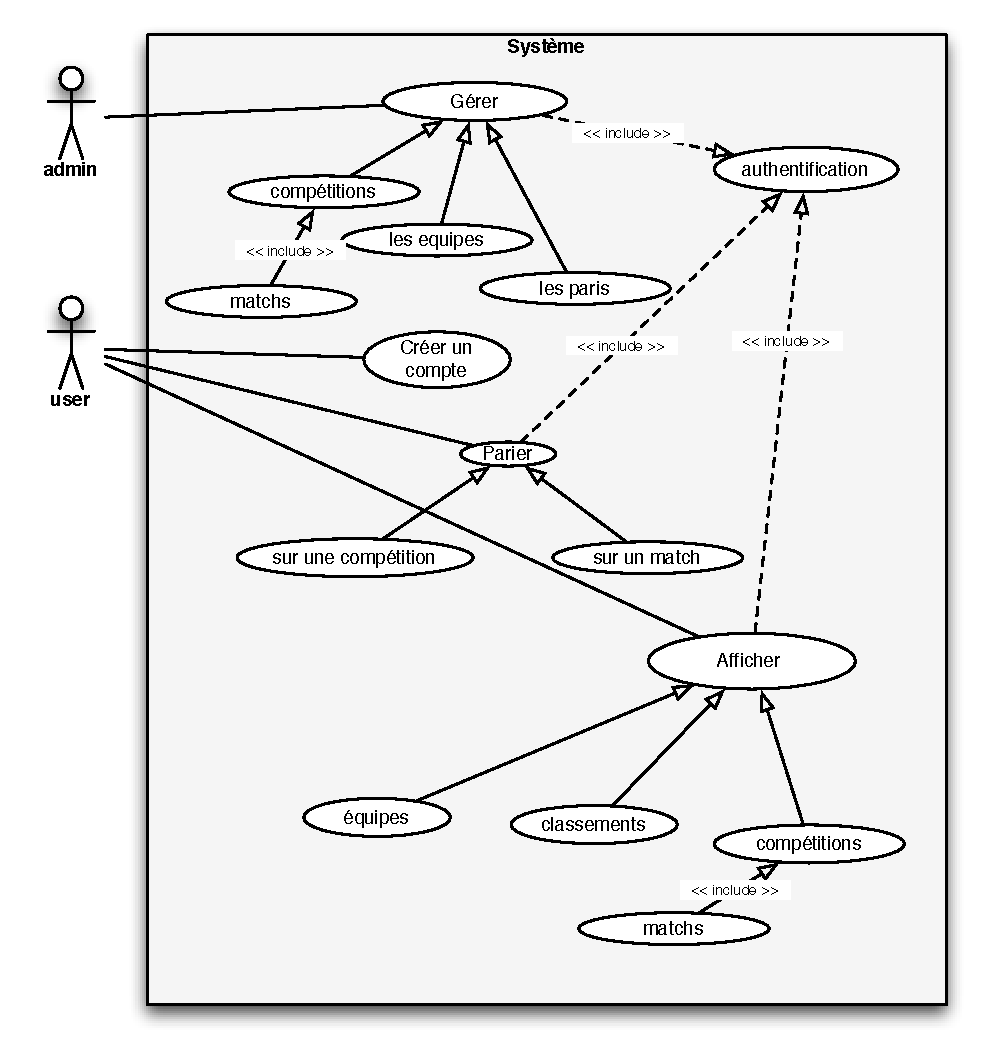
\includegraphics[width=12cm]{imgs/cas_utilisation-notitle.pdf}

Voici une liste des contrôleurs qui s'occupent d'effectuer les tâches décrites dans les cas d'utilisation ci-dessus.

\begin{description}
	\item[label] description
\end{description}
% \begin{description}
% 	\item[ajax_controller.rb] effectue la recherche sur les noms des équipes en fonction de ce que rentre l'utilisateur. La recherche est effectuée en AJAX.
% 	\item[application.rb] base de l'application, contient les informations sur la session en cours de l'utilisateur connecté sur le site
% 	\item[competitions_controller.rb] 
% \end{description}

% -----------------------------------------------------------------------------
\section{Base de données}
% -----------------------------------------------------------------------------

Avant de pouvoir commencer le développement du site, il a en premier lieu fallu concevoir le schéma de la base de données. La conception de ce schéma, dont le résultat final est visible sur la figure \ref{MDC}, a été faite en prenant en compte les différents cas d'utilisation vus au chapitre \ref{casUtilisation}.\\
\begin{figure}[!h]
	\begin{center}
			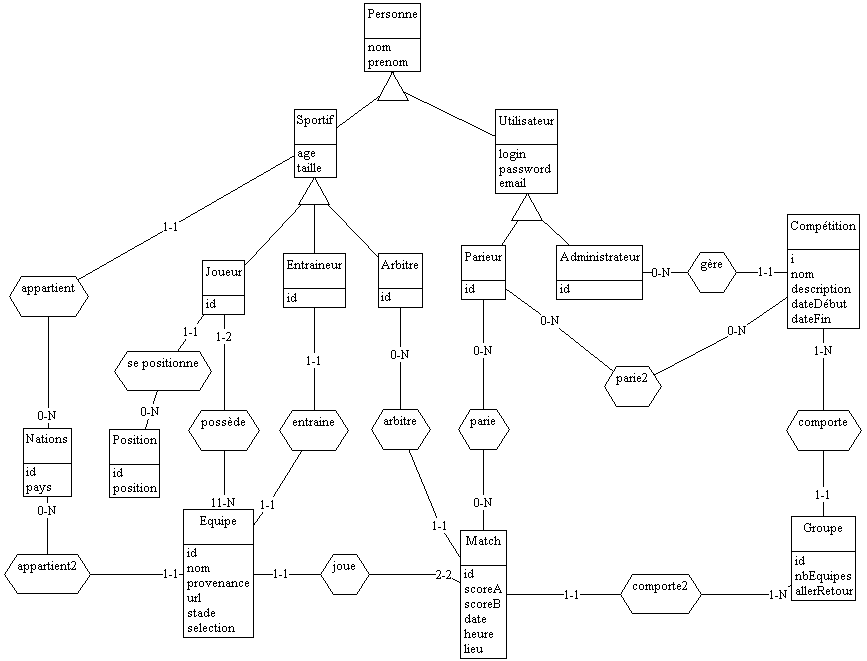
\includegraphics[width=12cm]{imgs/MDC.png}
			\caption{Modèle conceptuel de données}
			\label{MDC}
	\end{center}
\end{figure}

Il est possible de décomposer ce schéma, afin de mieux l'expliquer, dans les parties suivantes:
\begin{itemize}
	\item{Personnes}
	\item{Paris}
	\item{Compétitions}
	\item{Matchs}
\end{itemize}

\subsection{Personnes}
Cette partie du schéma se réfère à toutes les types de personnes existant dans la base de données. Comme il est possible de le voir sur le schéma, il existe cinq types de personnes:
\begin{itemize}
	\item{les joueurs;}
	\item{les entraîneurs;}
	\item{les arbitres;}
	\item{les parieurs;}
	\item{les administrateurs;\\}
\end{itemize}

Comme chacun de ses types possède un nom et un prénom, il a été décidé la création d'un type “Personne” dont tout le monde hérite. Néanmoins il est encore possible de diviser en deux catégories les cinq types de personnes énumérées ci-dessus. En effet, les types “Joueur”, “Entraîneur” et “Arbitre” possèdent en commun une taille, une date de naissance et une nationalité, la catégorie “Sportif” a donc été définie. Elle hérite donc du type “Personne” et est le type “parent” des joueurs, entraîneurs et arbitres.\\

Pour les deux types restants, c'est-à-dire, “Parieur“ et “Administrateur”, il est également possible de les regrouper dans la catégorie “Utilisateur” qui hérite de “Personne”. En effet, ils ont en commun un nom d'utilisateur, un mot de passe et un email.\\

Le schéma de la base de données de “RubyParis” possède donc de l'héritage, ce qui à priori est considéré un avantage en programmation, ne nous a pas convaincu dans ce cas. En effet, il est difficile de mettre en place un système d'héritage en base de données tel qu'il existe dans les langages de programmation. Il nous a donc fallu passer quelque temps à tester diverses façons de faire et les deux les plus plausibles sont, l'utilisation de “vues” dans la base de données et la création d'une seule table dans la base de données. Cette dernière façon de faire doit être couplée à un système d'héritage au niveau du modèle ce qui permet ensuite l'accès aux tables de manière héritée au niveau du code ruby.\\

Nous avons finalement opté pour la première méthode, c'est-à-dire, la création de cinq vues afin de pouvoir accéder plus facilement au contenu de ces cinq tables.

\subsection{Paris}
Il existe deux types de paris, le pari sur le résultat d'un match, c'est-à-dire le nom du gagnant du match ou le match nul, ou le vainqueur final d'une compétition. Cette gestion est gérée avec les deux relations “N à N”, “parie” et “parie2” visibles sur le schéma de la figure \ref{MDC}.\\

Au niveau de la base de données, il a fallu créer deux tables, “competitions\_parieurs” et “matchs\_parieurs”, contenant chacune un champ résultat afin de pouvoir gérer ces relations “N à N”. Dans le cas de “competitions\_parieurs”, c'est les paris sur le vainqueur final des compétitions qui est stocké dans le champ résultat. C'est donc directement l'identifiant de l'équipe. Par contre, dans le cas de “matchs\_parieurs”, c'est les résultats des matchs qui est stocké. Le champ résultat peut avoir trois valeurs différentes:
\begin{description}
	\item [1] {Indique que c'est l'équipe jouant à domicile qui gagne}
	\item [0] {Indique qu'il y a match nul}
	\item [2] {Indique que c'est l'équipe jouant à l'extérieur qui gagne\\}
\end{description}

Les paris sont uniquement effectués par les “Parieurs”.

\subsection{Compétitions}
La conception de la base de données a été pensée dans le sens de pouvoir être assez flexible sur les différents formats de compétitions de football existantes. Une compétition est donc décomposée en groupes qui contiennent des matchs.\\

Cette manière de faire permet de gérer les compétitions avec un classement final ou le vainqueur est celui possède le plus de points à la fin. En effet, il suffit de définir une compétition possédant un seul groupe avec une série de matchs. Il est également possible de définir une compétition avec des matchs à élimination directe, pour cela il suffit de créer une compétition possédant plusieurs groupes de deux équipes. Il va de soit qu'il est également possible de définir une compétition mélangeant les deux formats.

\subsection{Matchs}
Le match peut être considéré l'élément central de l'application. En effet, c'est autour du match que tout tourne et c'est ce dernier qui fait le lien entre les parieurs, les compétitions et la partie sportive.\\

Un match est donc composé de deux équipes qui possèdent des joueurs et un entraîneur, d'un arbitre et d'autres champs. Le match est ensuite lié aux parieurs, qui comme déjà mentionné peuvent parier sur le résultat, et à un groupe qui appartient à une compétition.

% -----------------------------------------------------------------------------
\section{Authentification}
% -----------------------------------------------------------------------------
Afin de pouvoir parier, il faut être inscrit sur le site et ensuite authentifié. Il en va de même pour les administrateurs du site qui doivent pouvoir se connecter et accéder aux différentes options de gestion.\\

Cette authentification est faite à l'aide d'un nom d'utilisateur (login) et d'un mot de passe (password). Ces informations sont stockées dans la table “Utilisateur” de la manière suivante:
\begin{description}
	\item [login] {Il est stocké sous forme de caractères.}
	\item [password] {Le mot de passe est également stocké sous forme de caractères, mais il est chiffré. En effet, lors de l'inscription de l'utilisateur, le mot de passe est chiffré avec l'algorithme SHA-1 avec un “sel” aléatoire de deux caractères. Le “sel” est ensuite concaténé avec le mot de passe et le tout est stocké dans le champs “password” dans la table.\\}
\end{description}

Lors de l'authentification, le mot de passe chiffré est récupéré dans la base de données grâce au nom d'utilisateur. Le “sel” concaténé au mot de passe est récupéré et l'opération de chiffrement décrite auparavant est effectuée sur le mot de passe entré par l'utilisateur avec le “sel” récupéré. Une fois ceci fait, les deux mots de passe chiffrés sont comparés et s'il sont identiques, l'authentification est réussie.\\

Une classe a été créé afin d'effectuer ces opérations. C'est la classe \verb!Hashpw! qui se trouve dans le répertoire \verb!helpers!.

% -----------------------------------------------------------------------------
\section{Ajax}
% -----------------------------------------------------------------------------

Nous avons utilisé AJAX pour la recherche d'équipe sur la home page. Ceci permet à l'utilisateur de taper quelques lettres d'une équipe, et les premières équipes contenant ces lettres seront affichées. Ensuite, en cliquant sur cette équipe, on affiche les informations la concernant. \\

Nous aurions pu utiliser AJAX qui est fournit par \texttt{Ruby On Rails}, mais nous avons plutôt opté pour JQuery. Pour effectuer ceci, nous avons utiliser Ruby On Rails pour générer les données, ainsi que JQuery. JQuery a été présenté lors de notre travail précédant et il était intéressant pour nous de l'intégrer dans notre projet. \\

Pour ceci, nous devons référencer la librairie JQuery que nous avons au préalable insérée dans \texttt{public/javascripts/jquery.js}. Ensuite, pour y faire référence, nous utilisons la méthode définie par ruby \texttt{javascript\_include\_tag "jquery"} dans notre modèle afin que le script soit importé. \\

Nous avons défini une action dans un contrôleur prévu à cet effet. C'est le contrôleur \texttt{ajax\_controller.rb} qui s'occupe de cela. Ensuite nous avons défini une vue qui affichait la liste des équipes. C'est la vue \texttt{liste\_ajax.rhtml}. Elle affiche simplement une liste des équipes trouvées par le contrôleur. \\

Il nous reste à écrire le code AJAX en JQuery qui permet d'interagir avec la vue citée ci-dessus. Voici le code :

\begin{lstlisting}
<script type="text/javascript">
  	// fonction pour AJAX en utilisant la librairie jQuery et ROR
   function lookup(inputString) {
      if(inputString.length == 0) {
         $('#suggestions').hide();
      } else {
         $.post("/ajax/liste_ajax", {eq: ""+inputString+""}, function(data){
            if(data.length >2) {
               $('#suggestions').show();
               $('#autoSuggestionsList').html(data);
            }
         });
      }
   } // lookup
   
   function fill(thisValue) {
      $('#inputString').val(thisValue);
      setTimeout("$('#suggestions').hide();", 200);
   }
  </script>
\end{lstlisting}

Cette méthode sera appelée lors de l'insertion de texte dans le champs prévu à cet effet. Il s'agit d'un champs de texte affiché sur la home page. Lorsqu'un caractère est tapé dans ce champs et que ce champs n'est pas vide, la fonction va envoyer ces informations (\texttt{\$.post()})  à la vue. C'est ensuite la fonction \texttt{function(data)} qui prend le relais. Si le contenu de la liste retournée n'est pas vide, nous allons afficher la fenêtre flottante des résultats et y insérer les données HTML contenant la liste des équipes trouvées.

% -----------------------------------------------------------------------------
\section{Conclusion}
% -----------------------------------------------------------------------------

Il est passionnant de découvrir un technologie comme Ruby On Rails. Elle comporte beaucoup d'avantages et que quelques inconvénients. Parmi les avantages citons la capacité de modifier le code source en fonction de la base de données très facilement, les support du modèle MVC, l'intégration d'autres “plugins” se fait facilement, et la simplicité mais la force du langage \texttt{Ruby} en font une plate-forme de développement très puissante et agréable. Comme inconvénients, la fait que le nombre d'hébergeurs soit encore trop faible, la structure peut paraître complexe au premier abords, le nombre de fichiers à manipuler est surprenant au début.\\

Mais dans l'ensemble, nous sommes très content d'utiliser \texttt{ROR} et espérons pouvoir l'utiliser encore prochainement sur un projet avec plus de temps à dispositions. 


\end{document}